\documentclass[letterpaper]{article}
\usepackage[spanish]{babel}
\usepackage{fixltx2e}
\usepackage{graphicx}
\usepackage[utf8]{inputenc}
\usepackage{hyperref}
\usepackage{mathtools}
\usepackage{numprint}
\usepackage{tabu}

\npthousandsep{\thinspace}
\npthousandthpartsep{}
\npdecimalsign{,}

\begin{document}

\title{Evaluación del informe\\``Generación de códigos únicos para
unidades geográficas"}
\author{Sylvain Lesage\\
\texttt{slesage@adsib.gob.bo}}
\date{\today}
\maketitle

\section{Antecedentes}

El Instituto Nacional de Estadísticas (INE) esta trabajando en una 
nueva codificación de los lugares, en particular localidades, 
comunidades y manzanos. El actual código tiene el problema de depender 
de la situación administrativa del lugar, por ejemplo el código 
actual contiene el código del departamento y del municipio. Es un 
problema en varias localidades o comunidades para las cuales la 
situación administrativa, en particular la dependencia a tal o tal 
municipio, no esta consensuada. Por esta razón, el INE decidió 
generar un nuevo código, basado únicamente en la ubicación 
geográfica del lugar, es decir la latitud y la longitud de un punto, 
que puede ser el centroide del territorio.

En el marco de las relaciones inter-institucionales entre el INE y la 
ADSIB, el equipo técnico del INE nos propuso revisar su propuesta de 
nuevo código. En este informe, describimos nuestra evaluación, y 
proponemos alternativas.

\section{Problemática}
\label{sec:problematica}

El nuevo código INE busca resolver el problema siguiente:

\begin{quote}
codificar la ubicación de un punto geográfico, de manera única para
un cierto nivel de precisión, en un número mínimo de caracteres.
\end{quote}

Algunas características deseables del código son:
\begin{itemize}
	\item código reversible: codificar un punto, y descodificar luego, 
	debe llevar a una aproximación buena del punto de origen, dentro
	del nivel de precisión exigido.
	\item código compacto: utilizar el número mínimo de caracteres, 
	que sean números o letras, para codificar la ubicación.
	\item precisión alta: reducir la superficie de las zonas de mismo 
	código a lo mínimo.\footnote{Hay que notar que el código no puede 
	ser único. En efecto, la codificación consiste a dividir el 
	territorio nacional, o sea una superficie continua, en un número 
	finito de códigos, cada código correspondiendo a una zona 
	definida. Más que buscar un hipotético código único, se trata de 
	definir el \emph{nivel de precisión} del código: por ejemplo, 
	¿que es la superficie de las zonas de mismo código? Un nivel de 
	precisión alto corresponde a una zona pequeña, por ejemplo: \(
	10\,\mathrm{m}\) por \(10\,\mathrm{m}\).}
	\item forma adecuada de las zonas de mismo código: puede ser un 
	cuadrado en el sistema latitud/longitud, un hexágono, un rectángulo,
	u otras formas. Lo más lógico es que la forma sea la más compacta 
	posible alrededor del centroide.
	\item nivel de precisión incremental: idealmente, los primeros
	caracteres del código expresan la ubicación a un nivel de precisión
	bajo, y cada nuevo carácter aumenta el nivel de precisión.
	\item simplicidad del cálculo: el cálculo debe ser lo más 
	simple, a partir de los datos más comunes para la ubicación de 
	puntos, es decir latitud y longitud en el sistema WGS84\footnote
	{WGS84 es el estándar utilizado en el sistema GPS, ver \url
	{https://en.wikipedia.org/wiki/World_Geodetic_System.}}
	\item simplicidad de los cálculos conexos: en particular, el 
	código debe ser diseñado de manera a facilitar el cálculo de 
	proximidad entre dos localidades.
	\item herramientas disponibles: una abundante lista de 
	herramientas compatibles con el código es una ventaja para su uso 
	masivo y para la conversión del actual código al nuevo código.
\end{itemize}

\section{Características de la propuesta de nuevo código INE \(z\)}

La propuesta de nuevo código proveída por el INE se encuentra en 
anexo. Lo anotaremos \(z\) en las ecuaciones.

\subsection{Definición del código \(z\)}

Dadas \(x\) y \(y\) las coordenadas de un punto en la proyección
cónica conforme de Lambert (PCCL)\footnote{Sistema Unico de
Información de la Tierra, \emph{Normas técnicas para la
administración de la información georeferenciada a nivel nacional}.
Resolución Ministerial Nº~338 del MDRAyMA, 2007, p.~33, \url{http://geo.gob.bo/?Normativa-SUNIT}}, el código \(z
\) esta definido\footnote{El documento base omite la adición de \(
\pi \) en el cálculo de \(\theta\). Lo añadimos para que nuestros
cálculos correspondan a los resultados proveídos por el equipo
técnico del INE.} por:

\[z = \lfloor r \exp{\theta} \rfloor\]

con

\[
\left\{
\begin{array}{l l}
r = \sqrt{x^2+y^2} \\
\theta = \arctan{\frac{y}{x}} + \pi
\end{array} \right.
\]

\subsection{Número de códigos \(z\) en Bolivia}

A partir del archivo de los límites de Bolivia\footnote{Límite
Nacional de Bolivia, en formato Shapefile, GADM: \url
{http://biogeo.ucdavis.edu/data/gadm2/shp/BOL_adm.zip}}, podemos
calcular los valores límites de las coordenadas \(x\) y \(y\) de
todos los puntos del territorio en la PCCL. La coordenada \(x\) se
encuentra en el intervalo \([\numprint{391248}\,\mathrm{m},
\numprint{1689926}\,\mathrm{m}]\) y la coordenada \(y\) en el
intervalo \([\numprint{119437}\,\mathrm{m},
\numprint{1583581}\,\mathrm{m}]\).

Podemos deducir el valor límite de las variables polares \(r\) y \(
\theta\). Tomar en cuenta que son valores límites, correspondiendo a 
las esquinas del \emph{bounding box} (cuadrado delimitado por \(
x_{min}\), \(x_{max}\), \(y_{min}\) y \(y_{max}\)) de Bolivia: no 
necesariamente existe un punto con estos valores de \(r\) y \(\theta
\). El radio \(r\) se encuentra en el intervalo \(
[\numprint{614506}\,\mathrm{m}, \numprint{1814299}\,\mathrm{m}]\) y 
el ángulo \(\theta\) en el intervalo \(
[\numprint{3.27}\,\mathrm{rad}, \numprint{4.44}\,\mathrm{rad}]\).

Según la formula de cálculo del código \(z\), esté crece con \(r\) y 
\(\theta\), por lo cual podemos calcular los valores límites del 
código \(z\) (con la misma advertencia: no necesariamente existe un 
punto en Bolivia que tenga estos valores extremos del código). Las 
estimaciones mínima y máxima del código \(z\) son respectivamente \(
\numprint{17493127}\) y \(\numprint{126692164}\). Por ende, podemos 
concluir que existe, en el territorio Boliviano, como estimación 
superior, \(\numprint{109199037}\) códigos diferentes.

El cuadro \ref{tab:variables} presenta un resumen de todos los valores.

\begin{table}
	\centering
	\begin{tabu} to \linewidth {|l|l|}
		\hline
		Variable & Valores \\
		\hline
		\(x\) & entre \(\numprint{391248}\,\mathrm{m}\) y \(\numprint{1689926}\,\mathrm{m}\) \\
		\(y\) & entre \(\numprint{119437}\,\mathrm{m}\) y \(\numprint{1583581}\,\mathrm{m}\) \\
		\hline
		\(r\) & entre \(\numprint{614506}\,\mathrm{m}\) y \(\numprint{1814299}\,\mathrm{m}\) \\
		\(\theta\) & entre \(3.27\,\mathrm{rad}\) y \(4.44\,\mathrm{rad}\) \\
		\hline
		código \(z\) & entre \(\numprint{17493127}\) y \(\numprint{126692164}\) \\
		número de códigos \(z\) & menos de \(\numprint{109199037}\) códigos diferentes \\
		\hline
	\end{tabu}
	\caption{Número de códigos \(z\) diferentes en Bolivia}
	\label{tab:variables}
\end{table}

\subsection{Precisión espacial del código \(z\)}

Tomando en cuenta que la superficie del territorio de Bolivia 
\footnote{según http://es.wikipedia.org/wiki/Bolivia} es 
aproximadamente de \(\numprint{1098581}\,\mathrm{km^{2}}\), podemos 
calcular que la superficie promedio del territorio correspondiendo a 
cada valor del código \(z\) es de \(\numprint{10060}\,\mathrm{m^{2}}
\), lo cual equivale un cuadrado de \(100\,\mathrm{m}\) de lado. 
Significa que para valor del código \(z\), existe una hectárea del 
territorio nacional donde todos los puntos comparten el mismo valor 
de \(z\), o sea donde el código \(z\) no permite discriminar entre 
los puntos incluidos. Podemos expresar este valor como el nivel de 
precisión del código \(z\). Los datos están presentados en el cuadro 
\ref{tab:precision}.

\begin{table}
	\centering
	\begin{tabu} to \linewidth {|l|l|}
		\hline
		Variable & Valores \\
		\hline
		superficie de Bolivia & \(\numprint{1098581}\,\mathrm{km^{2}}\) \\
		precisión del código  \(z\) & \(\numprint{10060}\,\mathrm{m^{2}}\), o sea una hectárea, como promedio\\
		\hline
	\end{tabu}
	\caption{Precisión espacial del código \(z\)}
	\label{tab:precision}
\end{table}

\subsection{Forma espacial de las zonas equi-código \(z\)}
\label{sec:forma_ine}

Podemos también calcular la forma de las áreas \emph{equi-código} \(z\). 
Los límites de estas áreas son definidos, para un valor específico 
de \(z\), y para los ángulos \(\theta\) correspondiendo a Bolivia, 
por los valores siguientes:

\[
\left\{
\begin{array}{l l}
r_{min} = z \exp{-\theta} \\
r_{max} = (z+1) \exp{-\theta}
\end{array} \right.
\]

Calculamos la geometría de las nueve áreas correspondiendo al código
de cada capital departamental de Bolivia. La figura \ref
{fig:areas_por_capital} representa estas áreas. Aparece claramente
que les áreas \emph{equi-código} forman \emph{franjas} muy estrechas
que cruzan toda Bolivia. Por ejemplo, el área que contiene el punto
central de La Paz mide \(\numprint{1224}\,\mathrm{km}\) de largo y
solamente \(\numprint{2.24}\,\mathrm{cm}\) de ancho en promedio (con
un ancho mínimo de \(\numprint{1.18}\,\mathrm{cm}\) y un ancho
máximo de \(\numprint{3.80}\,\mathrm{cm}\)). Su superficie es de \(
\numprint{19292}\,\mathrm{m^{2}}\), lo que equivale a un cuadrado de
\(\numprint{138}\,\mathrm{m}\) de lado. El detalle de estas medidas
para las nueve capitales de Bolivia se encuentra en el cuadro \ref
{tab:capitales}.

\begin{figure}[p]
	\centering
	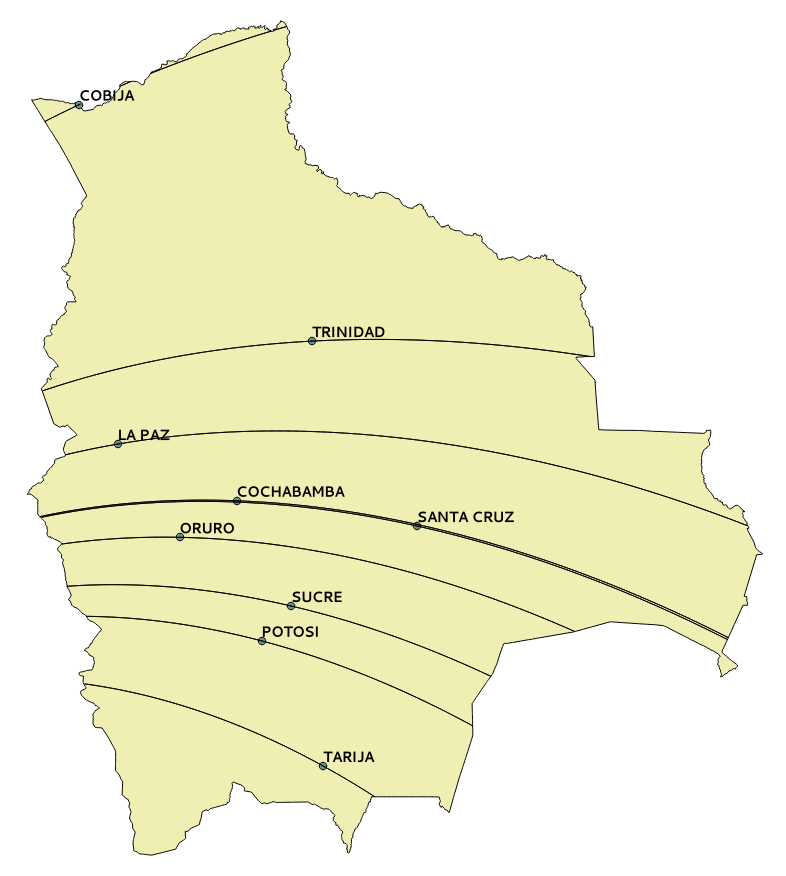
\includegraphics[width=0.5\textwidth]{resultados/area_equi_codigo_9_capitales.png}
	\caption{Área \emph{equi-código} para cada capital departamental de Bolivia. Nota: las áreas parecen líneas porque son extremadamente estrechas (\(\numprint{2.24}\,\mathrm{cm}\) en promedio)}
	\label{fig:areas_por_capital}
\end{figure}

\begin{table}
	\centering
	\begin{tabu} to \linewidth {|l|l|l|l|l|}
		\hline
		Capital & Superficie & Eq. precisión & Largo & Ancho (promedio) \\
		\hline
		Cobija & \(\numprint{3377}\,\mathrm{m^{2}}\) & \(\numprint{58}\,\mathrm{m}\) & \(\numprint{352}\,\mathrm{km}\) & \(\numprint{2.24}\,\mathrm{cm}\) \\
		Trinidad & \(\numprint{12957}\,\mathrm{m^{2}}\) & \(\numprint{113}\,\mathrm{m}\) & \(\numprint{983}\,\mathrm{km}\) & \(\numprint{2.24}\,\mathrm{cm}\) \\
		La Paz & \(\numprint{19292}\,\mathrm{m^{2}}\) & \(\numprint{113}\,\mathrm{m}\) & \(\numprint{1224}\,\mathrm{km}\) & \(\numprint{2.24}\,\mathrm{cm}\) \\
		Cochabamba & \(\numprint{21072}\,\mathrm{m^{2}}\) & \(\numprint{145}\,\mathrm{m}\) & \(\numprint{1244}\,\mathrm{km}\) & \(\numprint{2.24}\,\mathrm{cm}\) \\
		Oruro & \(\numprint{15302}\,\mathrm{m^{2}}\) & \(\numprint{145}\,\mathrm{m}\) & \(\numprint{919}\,\mathrm{km}\) & \(\numprint{2.24}\,\mathrm{cm}\) \\
		Sucre & \(\numprint{13106}\,\mathrm{m^{2}}\) & \(\numprint{114}\,\mathrm{m}\) & \(\numprint{760}\,\mathrm{km}\) & \(\numprint{2.24}\,\mathrm{cm}\) \\
		Potosí & \(\numprint{12907}\,\mathrm{m^{2}}\) & \(\numprint{113}\,\mathrm{m}\) & \(\numprint{701}\,\mathrm{km}\) & \(\numprint{2.24}\,\mathrm{cm}\) \\
		Tarija & \(\numprint{10864}\,\mathrm{m^{2}}\) & \(\numprint{104}\,\mathrm{m}\) & \(\numprint{540}\,\mathrm{km}\) & \(\numprint{2.24}\,\mathrm{cm}\) \\
		Santa Cruz & \(\numprint{21064}\,\mathrm{m^{2}}\) & \(\numprint{145}\,\mathrm{m}\) & \(\numprint{1241}\,\mathrm{km}\) & \(\numprint{2.24}\,\mathrm{cm}\) \\
		\hline
	\end{tabu}
	\caption{Área \emph{equi-código} para cada capital departamental de Bolivia}
	\label{tab:capitales}
\end{table}

A partir de la forma de las franjas, muy estrechas según el eje
norte-sur y muy anchas según el eje oeste-este, podemos entender una
característica del código \(z\): consiste, de manera aproximada, en
codificar el único dato de la latitud, obviando el dato de la
longitud. En efecto, de manera aproximada, el conocer el código \(z\)
permite encontrar con mucha precisión la latitud de todos los
puntos, pero impide totalmente conocer su longitud. El código es
entonces a un solo sentido: podemos generar un código a partir de un
punto, pero \emph{no se puede encontrar la ubicación precisa de un
punto a partir del código}.

La figura \ref{fig:areas_por_capital} y su acercamiento en la ciudad
de Santa Cruz (figura \ref
{fig:areas_por_capital_santacruz_cochabamba}) muestran que por
casualidad, las áreas \emph{equi-código} \(z\) de Santa Cruz y
Cochambamba casi se superponen, lo que significa que posiblemente
varios manzanos de Santa Cruz y de Cochabamba compartan el mismo
código.

\begin{figure}[p]
    \centering
    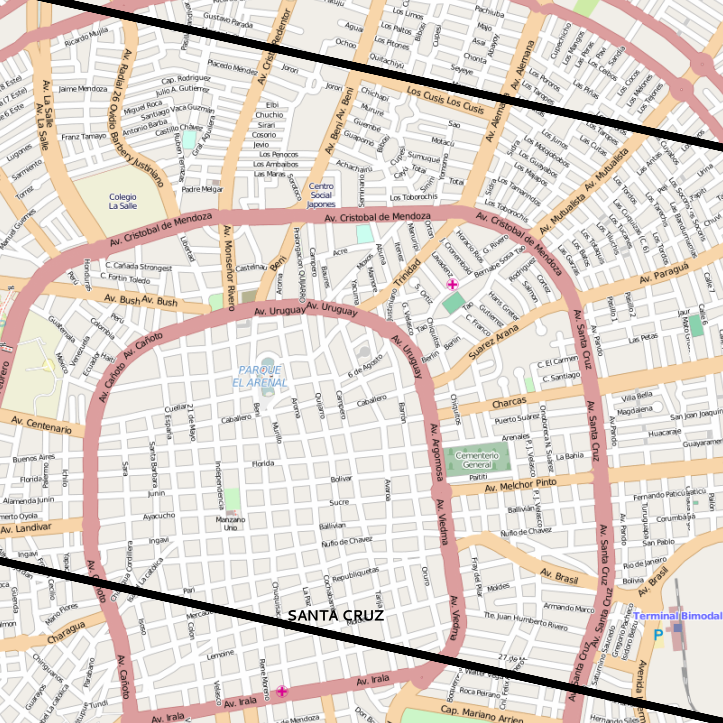
\includegraphics[width=0.5\textwidth]{resultados/area_equi_codigo_santacruz_cochabamba.png}
    \caption{Acercamiento sobre la ciudad de Santa Cruz para las áreas \emph{equi-código} para Santa Cruz y Cochabamba. Toda una franja de la ciudad de Santa Cruz (banda negra arriba) comparte el mismo código que la ciudad de Cochambamba}
    \label{fig:areas_por_capital_santacruz_cochabamba}
\end{figure}

\subsection{Otras características del código \(z\)}
\label{sec:otras_ine}

En la sección \ref{sec:problematica} definimos varios criterios de 
evaluación de una propuesta de código. En las secciones anteriores, 
detallamos los criterios de precisión y de forma de las zonas de mismo 
código. Evaluamos en esta sección los otros criterios para el código 
\(z\).

El código \(z\) esta compuesto únicamente de cifras, entre ocho y
nueve cifras. En la propuesta del INE, este número de cifras no es
configurable según el nivel de precisión deseado, es fijo y depende
de la formula de definición del código \(z\). Sin embargo, podemos
imaginar cambiar la definición para que sea configurable según un
parámetro entero \(n\) que aumentará el nivel de precisión, y con él
el tamaño del código:

\[z = \lfloor 10^{n} r \exp{\theta} \rfloor\]

El nivel de complejidad del cálculo de código es un poco elevado,
dado que, según la definición del código \(z\), el cálculo necesita
la transformación de las coordenadas del punto en la PCCL.

La proximidad de dos códigos \(z\) permite establecer una proximidad 
aproximativa en el eje norte-sur (ver la figura \ref
{fig:areas_por_capital}) pero no da indicios sobre la proximidad en 
el eje oeste-este. En un ejemplo extremo, dos puntos ubicados 
respectivamente sobre la frontera con Perú y sobre la frontera con 
Brazil pueden tener el mismo código \(z\).

Finalmente, por su recién invención, no existen herramientas para 
manejar el código \(z\).

\subsection{Resumen de las características del código \(z\)}

A continuación presentamos las características del código 
\(z\) de manera concisa:

\begin{itemize}
	\item criterio: Código \(z\){}
	\item descripción: inventado en 2014 por el equipo técnico del INE
	\item código para la Paz: 61220260
	\item descodificar: No. Preciso en latitud, pero no permite conocer la
	longitud del punto original 
	\item tamaño del código: 8 o 9 cifras (10 posibilidades por carácter)
	\item superficie equi-código con 9 caracteres (La Paz): \(\numprint{19292}\,\mathrm{m^{2}}\), 
		equivalente a un cuadrado de \(\numprint{113}\,\mathrm{m}\) de lado
	\item forma equi-código (La Paz): una franja de \(\numprint{1224}\,\mathrm{km}\) por 
		\(\numprint{2.24}\,\mathrm{cm}\)
	\item configurar precisión: no esta previsto, pero se podría implementar (ver \ref{sec:otras_ine})
	\item cálculo del código: necesita reproyectar de WGS84 en Lambert
	\item cálculo de proximidad: fácil en un eje norte-sur, pero imposible en un eje oeste-este
	\item herramientas disponibles: ninguna
\end{itemize}

\section{Códigos alternativos}

La problemática expuesta en la sección \ref{sec:problematica} no es 
nueva y ha sido estudiada desde varias décadas, resultando en varias 
definiciones de códigos, utilizados en varios ámbitos. En las
siguiente subsecciones presentamos tres de los códigos más 
utilizados.

\subsection{Características del código Geohash}

\begin{itemize}
	\item criterio: código GeoHash\footnote{ver \url{http://en.wikipedia.org/wiki/Geohash}}
	\item descripción: código inventado en 2008, para el servicio web \url{http://geohash.org}
	\item código para la Paz: 6mpd1mz3n 
	\item descodificar: si: se encuentra el punto original con una 
		precisión que depende del número de caracteres. 
	\item tamaño del código: variable - letras y cifras (36 
		posibilidades por carácter) 
	\item superficie equi-código con 9 caracteres (La Paz): 
		\(\numprint{21}\,\mathrm{m^{2}}\), 
		equivalente a un cuadrado de \(\numprint{4.6}\,\mathrm{m}\) de lado 
	\item forma equi-código (La Paz): rectángulo: 
		\(\numprint{4.7}\,\mathrm{m}\) (norte-sur) por 
		\(\numprint{4.5}\,\mathrm{m}\) (oeste-este) 
	\item configurar precisión: sí, cada 
		carácter aumenta el nivel de precisión\footnote{ver 
		\url{http://en.wikipedia.org/wiki/Geohash\#Worked_example}} 
	\item cálculo del código: muy rápido, solo es la codificación en
		base32 de la latitud y longitud 
		cálculo de proximidad: no es lo más adecuado\footnote{ver 
		\url{http://en.wikipedia.org/wiki/Geohash\#Limitations}} 
	\item herramientas disponibles: existen librerías para 15 lenguajes\footnote{ver 
		\url{http://en.wikipedia.org/wiki/Geohash\#External_links}}
		entre ellos los más utilizados: python, javascript, java, php,
		etc.
\end{itemize}

\subsection{Características del código MGRS}

\begin{itemize}
	\item criterio: código MGRS (Military grid reference system)\footnote{ver 
		\url{http://en.wikipedia.org/wiki/Military_grid_reference_system}} 
	\item descripción: código inventado y utilizado en un contexto
		militar por el OTAN, y utilizado desde 2001 en un marco civil en
		Estados Unidos bajo el nombre USNG (United States National Grid)
	\item código para la Paz: 19KEB9276 
	\item descodificar: si: se encuentra el punto original con una 
		precisión que depende del número de caracteres. 
	\item tamaño del código: variable - 5 letras y cifras, luego pares
		de cifras 
	\item superficie equi-código con 9 caracteres (La Paz): 
		\(\numprint{1000000}\,\mathrm{m^{2}}\), 
		equivalente a un cuadrado de \(\numprint{1000}\,\mathrm{m}\) de lado 
	\item forma equi-código (La Paz): rectángulo: 
		\(\numprint{1000}\,\mathrm{m}\) (norte-sur) por 
		\(\numprint{1000}\,\mathrm{m}\) (oeste-este) 
	\item configurar precisión: sí, cada dos 
		cifras dividen la superficie por 100 (o el lado del cuadrado 
		por 10)\footnote{ver 
		\url{http://en.wikipedia.org/wiki/Military_grid_reference_system}} 
	\item cálculo del código: necesita hacer una proyección en UTM 
	\item cálculo de proximidad: no se encontraron datos 
	\item herramientas disponibles: librerías GeographicLib y 
		GeoConvert/mgrs en 9 lenguajes\footnote{ver 
		\url{https://pypi.python.org/pypi/mgrs} para python} 
\end{itemize}

\subsection{Características del código MLOCS}

\begin{itemize}
	\item criterio: código MLocS (Maidenhead Locator System)\footnote{ver 
		\url{http://en.wikipedia.org/wiki/Maidenhead_Locator_System}} 
	\item
		descripción: código inventado y utilizado por los
		radioaficionados desde 1980.
	\item código para la Paz: FH53WM32 
	\item descodificar: si: se encuentra el punto original con una 
		precisión que depende del número de caracteres. 
	\item tamaño del código: variable, con pares sucesivas de letras y
		cifras 
	\item superficie equi-código con 8 caracteres (La Paz): 
		\(\numprint{1628640}\,\mathrm{m^{2}}\), 
		equivalente a un cuadrado de \(\numprint{1276}\,\mathrm{m}\) de lado 
	\item forma equi-código (La Paz): rectángulo: 
		\(\numprint{1837}\,\mathrm{m}\) (norte-sur) por 
		\(\numprint{886}\,\mathrm{m}\) (oeste-este) 
	\item configurar precisión: sí, cada dos 
		cifras aumentan la precisión (un vez dividiendo por 10 con
		un par de cifra, la otra por 24 con un par de letras) 
	\item cálculo del código: rápido porque opera directamente sobre
		las divisiones en grados, minutos, etc. de latitud y longitud 
	\item cálculo de proximidad: no encontrado 
	\item herramientas disponibles: librerías en python (mlocs), perl, 
		y esta implementado en varios dispositivos GPS 
\end{itemize}

\section{Comparación de la precisión de los cuatro códigos}
\label{sec:precision}

Después de haber presentado algunas características de los códigos 
Geohash, MGRS y MLOCS, hacemos una comparación de la precisión de las 
zonas equi-código (o sea, la distancia máxima entre el punto original 
que sirvió a generar el código y el punto obtenido descodificando). 
Los resultados están desplegados en la figura 
\ref{fig:precision_codigos}.

\begin{figure}[p]
    \centering
    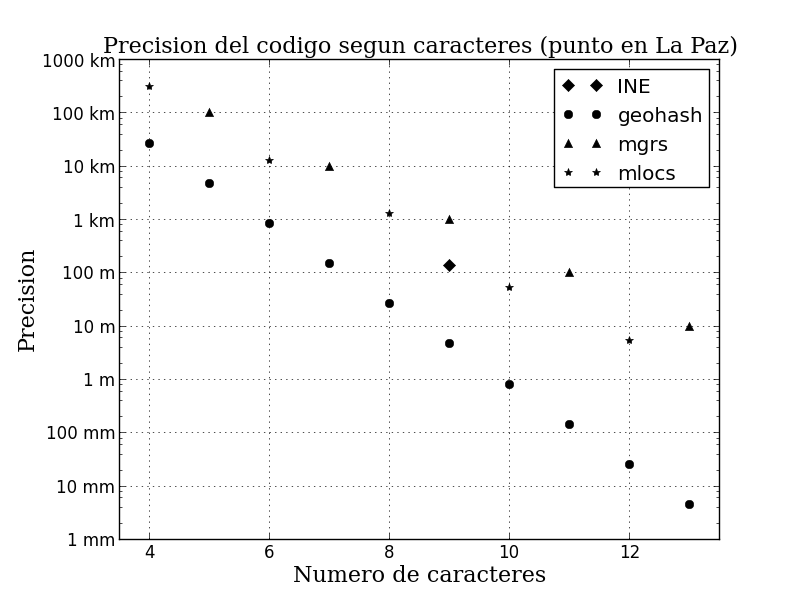
\includegraphics[width=0.8\textwidth]{resultados/precision_codigos.png}
    \caption{Precisión de los cuatro códigos (INE, Geohash, MGRS, 
    MLOCS) para el centro de La Paz, según el número de caracteres 
    en el código.}
    \label{fig:precision_codigos}
\end{figure}

La primera observación es que para los tres códigos Geohash, MGRS y 
MLOCS, la precisión aumenta (o sea la distancia entre puntos 
disminuye) cuando el número de caracteres aumenta. A notar: la 
escala para el valor de la precisión es logarítmica. Implica que el 
aumento de precisión del código Geohash, por ejemplo, que 
corresponde a una línea recta en la escala logarítmica, es constante 
en ordenes de magnitud. Así, añadir 4 caracteres al código Geohash 
se traduce por una división por 1000 de la distancia máxima entre 
puntos. El código \(z\) no prevé configurar el número de caracteres, 
así que no podemos hacer el mismo análisis para este código. 

Segundo, aparece claramente que el código Geohash tiene la mejor 
precisión entre los cuatro códigos, a número de caracteres igual. La 
precisión del Geohash en comparación con los otros es de un orden de 
magnitud entre 10 y 100. Se debe, naturalmente, al uso de cifras y 
letras para caracteres, o sea 36 valores posibles por carácter, a 
comparar, por ejemplo para el código \(z\) que solo contiene cifras, 
con 10 valores por carácter, o sea un potencial de compresión 3.6 
veces más bajo.

Tercero, vemos que el código Geohash permite elegir cualquier número 
de caracteres (de 4 a 13 en la figura), mientras el código \(z\) tiene 
un número de caracteres fijo (8 o 9 según el punto), mientras el 
código MGRS debe tener un número de caracteres impar (5, 7, 9, 11, 
13), y el código MLOCS un número de caracteres par (4, 6, 8, 10, 12).

\section{Comparación de los puntos duplicados para los cuatro códigos}

El equipo técnico del INE nos proveyo una lista de 86538 puntos
(localidades y manzanos) con los datos de latitud y longitud.
Aplicamos los cuatro códigos sobre esta lista de puntos, y buscamos
el número de duplicados, es decir el número de puntos que comparten
el mismo código con por lo menos un otro punto. Los resultados se
encuentran en el cuadro \ref{tab:duplicados}.

\begin{table}
	\centering
	\begin{tabu} to \linewidth {|l|l|l|l|l|}
		\hline{}
		Caracteres & \(z\) & Geohash & MGRS & MLOCS \\
		\hline
		1 & - & 1 / 86538 & - & - \\
		\hline
		2 & - & 7 / 86532 & - & 4 / 86535 \\
		\hline
		3 & - & 64 / 86475 & - & - \\
		\hline
		4 & - & 1103 / 85436 & - & 64 / 86475 \\
		\hline
		5 & - & 11102 / 75437 & 149 / 86390 & - \\
		\hline
		6 & - & 27926 / 58613 & - & 8045 / 78494 \\
		\hline
		7 & - & 52210 / 34329 & 4524 / 82015 & - \\
		\hline
		8 & - & 83660 / 2879 & - & 29527 / 57012 \\
		\hline
		9 & 86538 / 0 & 86522 / 17 & 26861 / 59678 & - \\
		\hline
		10 & - & 86526 / 13 & - & 83596 / 2943 \\
		\hline
		11 & - & 86531 / 8 & 64985 / 21554 & - \\
		\hline
		12 & - & 86537 / 2 & - & 86525 / 14 \\
		\hline
		13 & - & 86538 / 0 & 86436 / 103 & - \\
		\hline
	\end{tabu}
	\caption{Número de códigos diferentes / Número de duplicados, entre las manzanas y localidades de Bolivia}
	\label{tab:duplicados}
\end{table}

Podemos ver que para los tres códigos Geohash, MGRS y MLOCS, el
número de puntos duplicados disminuye con el número de caracteres
del código. Es totalmente lógico, dado que la precisión del código
aumenta con el número de caracteres (ver la sección \ref
{sec:precision}). De hecho, si calculamos el Geohash con un solo
carácter, el resultado es siempre lo mismo: "6", y entonces todos
los códigos son duplicados. En efecto la zona equi-código en este
caso contiene el territorio de Bolivia por completo, porque la
precisión es mínima (un solo carácter implica dividir la superficie
del globo terráqueo en solo 36 zonas).

Cruzando los datos del cuadro \ref{tab:duplicados} con los datos de
la figura \ref{fig:precision_codigos}, podemos notar, por ejemplo,
que los 17 puntos duplicados con el código Geohash de 9 caracteres
corresponden a zonas de menos de 10 metros de tamaño. En este caso,
hablando de manzanos y localidades, dos puntos ubicados a menos de
10 metros de distancia obviamente corresponden a la misma ubicación,
y entonces es correcto que el código sea el mismo.

Sin embargo, podemos notar que el código \(z\) es diferente para los
86538 puntos, aunque, como lo hemos notado anteriormente, varios
puntos corresponden exactamente a la misma ubicación, aunque sus
coordenadas sean ligeramente diferentes (menos de 10 metros). Eso se
explica por la forma de las zonas equi-código para el código \(z\)
(ver la sección \ref{sec:forma_ine}), que son franjas que cruzan
todo el país en el eje oeste-este, pero con un ancho de solamente 2
centímetros en el eje norte-sur. La diferencia de precisión en la
latitud de los puntos que deberían ser duplicados, superior a estos
2 centímetros (pero inferior a 10 metros) explica porque tienen
códigos \(z\) diferentes. Significa entonces que el código \(z\) no
permite reconocer que dos puntos corresponden a la misma unidad
territorial (manzano, comunidad) si difieren mínimamente (por más de
2 centímetros) en su valor de latitud.

Retomando el ejemplo de la figura \ref
{fig:areas_por_capital_santacruz_cochabamba}, significa que
posiblemente, dos puntos ubicados en la misma casa en Cochabamba
tengan códigos \(z\) diferentes, mientras comparten su código con
una otra casa ubicada en Santa Cruz. Falla el código \(z\) en
reconocer dos puntos en la misma casa, y genera duplicados entre
puntos totalmente separados geográficamente.

\section{Conclusión y recomendaciones}



\end{document}
